%% 
%% This is file ejmcls.ltx - generated with MakeDist v1.0, by M. Reed 
%% 
 
\documentclass{article}

\usepackage[utf8]{inputenc}
\usepackage{lmodern}


\usepackage{geometry}                		% See geometry.pdf to learn the layout options. There are lots.
\geometry{letterpaper}                   		% ... or a4paper or a5paper or ... 
%\geometry{landscape}                		% Activate for for rotated page geometry
%\usepackage[parfill]{parskip}    		% Activate to begin subsubsections with an empty line rather than an indent
\usepackage{graphicx}				% Use pdf, png, jpg, or eps§ with pdflatex; use eps in DVI mode
								% TeX will automatically convert eps --> pdf in pdflatex		
\usepackage{fancyhdr}
\usepackage{amssymb}
\usepackage{dsfont}
\usepackage{amsmath}
\usepackage{pgfplots}
\usepackage{tikz}
\usepackage{enumerate}
\usepackage{quoting}
\usepackage{amsthm}

\usetikzlibrary{patterns}
\usetikzlibrary{decorations.text}
\usetikzlibrary{decorations.pathmorphing}

\usepackage{caption}
\usepackage{subfig}
%\usepackage{subcaption}
\usepackage{geometry}
%\geometry{top=2cm, bottom=2cm, left=2cm, right=2cm}
\geometry{margin=2cm}

\author{Gil-Arnaud Coche}
%\date{}							% Activate to display a given date or no date


\tikzset{
  pics/carc/.style args={#1:#2:#3}{
    code={
      \draw[pic actions] (#1:#3) arc(#1:#2:#3);
    }
  }
}



\numberwithin{equation}{section}

\setlength{\parindent}{0in}

\definecolor{awesomePurple}{rgb}{0.55, 0.42, 1}

\begin{document}

\newtheorem{hyp}{Hypothese}
\newtheorem*{hyp*}{Hypothese}

\pgfdeclarepatternformonly[/tikz/radius,\thickness,\size]{rings}
{\pgfpoint{-0.5*\size}{-0.5*\size}}
{\pgfpoint{0.5*\size}{0.5*\size}}
{\pgfpoint{\size}{\size}}
{
  \pgfsetlinewidth{\thickness}
  \pgfpathcircle\pgfpointorigin{\pgfkeysvalueof{/tikz/radius}}
  \pgfusepath{stroke}
}
\newdimen\thickness
\tikzset{
  radius/.initial=4pt,
  size/.store in=\size, size=20pt,
  thickness/.code={\thickness=#1},
  thickness=0.75pt
}

\newcommand{\W}{\mathcal{W}}
\newcommand{\B}{\mathcal{B}}
\newcommand{\diff}{\textnormal{d}}

\title{Allocation optimale avec consommation du capital.}

\author{Gil-Arnaud Coche}
\maketitle

On se donne un intervalle de temps de $K$ périodes discrètes et de durée $\delta t$. On va chercher à savoir quelle serait l'allocation optimale entre un actif risqué et un actif sans risque sachant que l'on consomme une partie de ce capital à chaque itération. Le portefeuille considéré sera autofinancé et de mise initiale $W_0$.

\section{Le modèle.}

\subsection{Les actifs}

On considère donc que l'on dispose deux actifs, l'un risqué que l'on nommera $x$ et l'autre sans risque que l'on nommera $x^0$. Pour simplifier la présentation,
\begin{itemize}
\item les rendements de l'actif risqué sont i.i.d. et ont une dynamique gaussienne simple
\begin{equation}
\mu_k = \frac{x_{k + 1} - x_k}{x_k} = m + \sigma \epsilon_k
\end{equation}
où $\epsilon_k\sim\mathcal N(0, 1)$;
\item les rendements de l'actif sans risque sont constants et égaux à $r$.
\end{itemize}


Ces hypothèses sont très fortes, néanmoins elles offrent un cadre intéressant pour se donner une idée rapide des enjeux de l'optimisation.\\

\subsection{Bilans de richesse}

\subsubsection{Entre deux sous-périodes $k$ et $k + 1$}

Pour écrire convenablement la variation de richesse entre deux périodes $k$ et $k + 1$ du portefeuille autofinancé, observons la figure \ref{fig:flux-de-richesse} de la page \pageref{fig:flux-de-richesse}. 
\begin{itemize}
\item En $k$, le portefeuille contient une richesse $\W_k$.\\

En $k^+$, les valeurs $\psi_k$ et $\psi_k^0$ sont investies respectivement dans l'actif risqué\footnote{On détient donc $\psi_k/x_k$ unités en cet actif.} et l'actif sans risque et la consommation pour la période à venir demande de retirer $c_k$ au capital courant en $k^+$. L'exposant $+$ est indiqué pour insister sur le fait que le décompte à lieu après l'enregistrement de la richesse $\W_k$ en $k$.\\

Le portefeuille contient donc en $k^+$ la richesse
$$
\W_k - c_k = \psi_k + \psi_k^0
$$
en début de période.

\item En $k + 1$, l'actif risqué a varié avec le rendement $\mu_k$ et l'actif sans risque avec le rendement $r$. Avant d'écrire le bilan, il est à noter que \\

Le portefeuille contient donc alors la richesse en fin de période
$$
\W^-_{k+1} = (1 + \mu_k)\psi_k + (1 + r)\psi_k^0
$$

Un exposant $-$ est ajouté à l'expression du dessus car il indique que la valeur est celle avant l'enregistrement en $k + 1$. Néanmoins, comme nous considérons que le portefeuille est \textbf{autofinançant} l'exposant est oublié dans la suite.\\

La richesse $\W_{k + 1}$ est donc strictement égale à l'expression de $\W_{k + 1}^-$ ci-dessus.

\end{itemize}

\begin{figure}[h!]
\centering
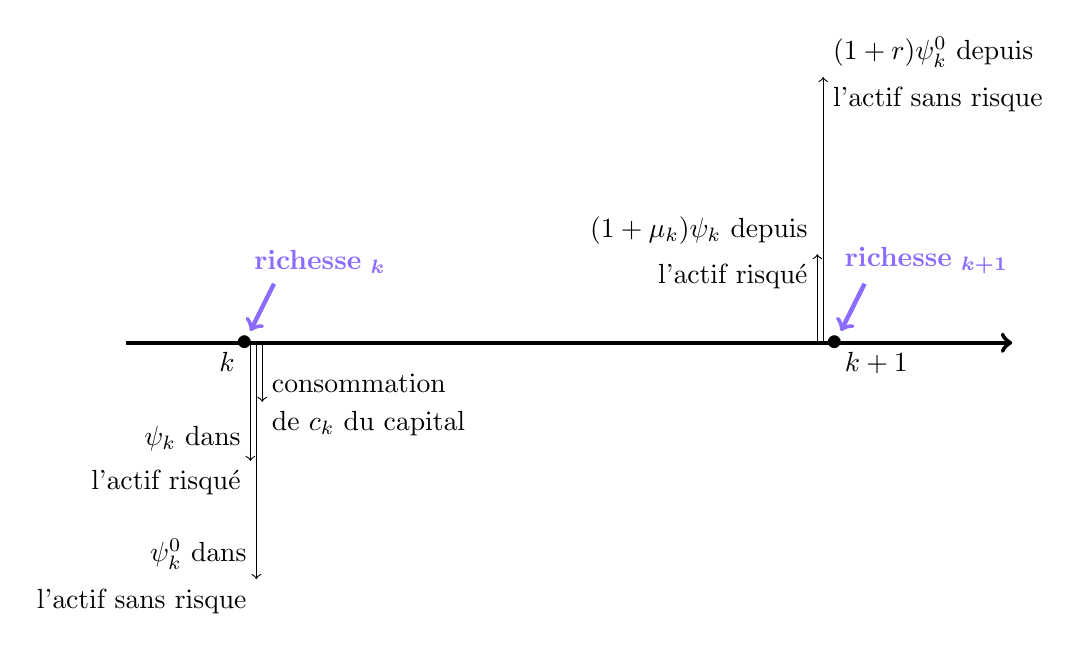
\begin{tikzpicture}[scale = .75]
\draw[->, ultra thick] (-2, 0) -- (13, 0);

\node at (0, 0) {\large $\bullet$};
\node at (0, 0) [below left] {$k$};
\node at (0, 1) [above right] {\color{awesomePurple}\textbf {richesse} $\boldsymbol {\W_{k}}$};
\draw [->, ultra thick, awesomePurple] (.5, 1) -- (0.1, .2);

\node at (10, 0) {\large$\bullet$};
\node at (10, 0) [below right] {$k + 1$};
\node at (10, 1) [above right] {\color{awesomePurple}\textbf {richesse} $\boldsymbol {\W_{k+1}}$};
\draw [->, ultra thick, awesomePurple] (10.5, 1) -- (10.1, .2);

\draw[->] (0.1, 0) -- (0.1, - 2);
\node at (0.1, -2) [above left] {$\psi_k$ dans};
\node at (0.1, -2) [below left] {l'actif risqué};

\draw[->] (.2, 0) -- (.2, - 4);
\node at (.2, -4) [above left] {$\psi_k^0$ dans};
\node at (.2, -4) [below left] {l'actif sans risque};

\draw[->] (.3, 0) -- (.3, - 1);
\node at (.3, -1) [above right] {consommation};
\node at (.3, -1) [below right] {de $c_k$ du capital};


\draw[->] (9.7, 0) -- (9.7, 1.5);
\node at (9.7, 1.5) [above left] {$(1 + \mu_k)\psi_k$ depuis};
\node at (9.7, 1.5) [below left] {l'actif risqué};

\draw[->] (9.8, 0) -- (9.8, 4.5);
\node at (9.8, 4.5) [above right] {$(1 + r)\psi_k^0$ depuis};
\node at (9.8, 4.5) [below right] {l'actif sans risque};

\end{tikzpicture}
\caption{Les flux de richesse entre deux périodes $k$ et $k + 1$.}
\label{fig:flux-de-richesse}
\end{figure}

Le bilan entre $k + 1$ et $k$ se formule donc en
\begin{equation}
\W_{k + 1} - (1 + r)\W_k = (\mu_k - r) \psi_k - (1 + r)c_k
\end{equation}


\subsubsection{Entre le début du placement et la fin de la période d'investissement $K$}

De l'équation précédente on peut aisément déduire a variation totale de richesse pour l'investisseur en introduisant la richesse actualisée $\tilde \W_k$ telle que $(1 + r)^k\tilde\W_k = \W_k$. La variation de richesse actualisée d'une période à l'autre est égale à 
$$
\tilde\W_{k + 1} - \tilde\W_k = (\mu_k - r) \frac{\psi_k}{(1 + r)^{k+1}} - \frac{c_k}{(1 + r)^k}.
$$

A chaque instant $k$, on a une somme télescopique qui mène, tous calculs faits, à
\begin{equation}
\tilde\W_k =  W_0 + \sum_{l=0}^{k - 1}(\mu_l - r) \frac{\psi_l}{(1 + r)^{l+1}} - \sum_{l=0}^{k - 1} \frac{c_l}{(1 + r)^l}
\end{equation}

\textbf{\color{awesomePurple}La richesse actualisée est la somme d'une position longue en le portefeuille d'investissement en actif risqué et actif sans risque et d'une position courte en un bond de coupon variable $c_k$.}


\section{Les objectifs de l'investissement.}

Dans cette illustration, on va considérer que l'investisseur est un petit porteur averse au risque qui souhaite maximiser ses revenus sans pour autant prendre des risques inconsidérés.\\

\subsection{Benchmark d'un investisseur totalement averse au risque}

Si cet investisseur a une aversion maximale au risque, il n'investirait rien dans l'actif risqué et en bout de période, il aurait
$$
\tilde\W_K = 0 = W_0 - \sum_{k=0}^{K - 1} \frac{c^0_k}{(1 + r)^k}.\\
$$

Puisque l'investisseur souhaite maximiser le capital $c_k$ dont il dispose à chaque période, la répartition optimale est celle qui assure des coupons de valeur
$$
\frac{c^0_k}{(1 + r)^k} = \frac{\W_0}{K}.
$$

\textbf{\color{awesomePurple}Un benchmark utile est donc de considérer la stratégie totalement averse au risque qui assurerait de disposer à chaque période du capital
\begin{equation}
c_k^0 = \left( 1 + r \right)^k\frac{\W_0}{K}.
\end{equation}}

\subsection{Maîtriser les revenus du bond de coupons $c_k$}

Tout l'intérêt du placement en actifs risqué et sans risque est de pouvoir bénéficier des rendements de marchés. Avec une stratégie  bien structurée, l'investisseur peut augmenter l'espérance de ses coupons futurs $c_k$.\\ 

Mathématiquement, cela peut s'obtenir en fixant comme objectif de maximisation la valeur actualisée des flux de ces versements
\begin{equation}
\B_K = \sum_{k=0}^{K - 1} \frac{c_k}{(1 + r)^k}
\end{equation}
avec pour variables de l'optimisation les valeurs des coupons versés $c_k$.\\

\textbf{\color{awesomePurple}Une stratégie gagnante pour l'investisseur est une stratégie qui lui permettra de pouvoir assurer un flux de coupons $c_k$ qui sera supérieur à $c^0_k$.}

\subsection{Maîtriser les pertes des investissements risqués}

En l'occurence, son soucis principal est d'éviter d'avoir un capital à chaque période qui soit inférieur à celui qu'il obtiendrait avec la stratégie sans risque. Autrement dit, on souhaite toujours avoir
$$
\tilde \W_k\geq\tilde\W^0_k
$$
où 
$$
\tilde\W^0_k = \left( 1 - \frac{k}{K} \right)W_0
$$
est la richesse en $k$ obtenue avec la stratégie sans risque.
\\

Mathématiquement, cela s'écrit plus précisément comme
\begin{equation}
\mathds P\left(\forall 1\leq k\leq K,\ \tilde \W_k\geq\tilde\W^0_k\right) = 1 - \alpha
\end{equation}
avec $\alpha$ une probabilité fixée par l'investisseur en fonction de son aversion au risque. Si $\alpha = 0$, l'investisseur est averse au risque et on devrait donc retrouver le versement du coupon $c_k^0$.\\

\textbf{\color{awesomePurple}Une stratégie gagnante pour l'investisseur devra donc assurer qu'une proportion $1 - \alpha$ de chemins pris des prix de l'actif risqué, assure en chaque période une richesse supérieure à celle obtenue par la stratégie sans risque.}

\subsection{Contraintes structurelles au placement}

Les placements à découverts sont interdits et aucun capital n'est injecté au fur et à mesure. On a donc

\begin{equation}
\mathds P\left(\left(1 + r\right)^k\tilde\W_k\geq \psi_k + c_k\right) = 1\ \ \textnormal{et}\ \ \psi_k\geq0, c_k\geq 0
\end{equation}

\textbf{\color{awesomePurple}Une stratégie gagnante pour l'investisseur est une stratégie qui ne placera dans l'actif sans risque que les fonds disponibles une fois la paiment du coupon et le placement en actif risqué effectué.}


\subsection{Formulation du problème d'optimisation}

On a finalement le problème mathématique suivant pour aller chercher la stratégie optimale d'allocation des ressources de l'investisseur.

\begin{equation}
\begin{split}
&\max_{\psi_k, c_k}\sum_{k=0}^{K - 1} \frac{c_k}{(1 + r)^k}\\
\\
\textnormal{s.c. }&\tilde\W_k =  W_0 + \sum_{l=0}^{k - 1}(\mu_l - r) \frac{\psi_l}{(1 + r)^{l+1}} - \sum_{l=0}^{k - 1} \frac{c_l}{(1 + r)^l}\\
&\mathds P\left(\forall 1\leq k\leq K,\ \tilde \W_k\geq \left( 1 - \frac{k}{K} \right)W_0\right) = 1 - \alpha\\
&\mathds P\left(\tilde\W_k\geq \frac{\psi_k + c_k}{\left(1 + r\right)^k}\right) = 1,\ \forall 1\leq k\leq K\\
&\psi_k\geq0\\
&c_k\geq 0
\end{split}
\end{equation}

\end{document}